\documentclass[11pt]{article}
\usepackage{tikz}
\usetikzlibrary{positioning,chains,fit,shapes,calc,graphs, shapes.multipart, calc}

    \tikzstyle{bplus}=[rectangle split, rectangle split horizontal,rectangle split ignore empty parts,draw, fill=white]
    \tikzstyle{every node}=[bplus]
    \tikzstyle{level 1}=[sibling distance=45mm]
    \tikzstyle{level 2}=[sibling distance=18mm]
    
\begin{document}
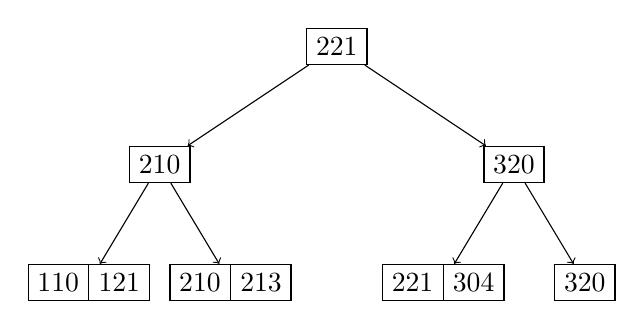
\begin{tikzpicture}
	\node {221} [->]
	child {node {210} 
		child {node {110 \nodepart{two} 121}}
		child {node {210 \nodepart{two} 213}}} 
	child {node {320} 
		child {node {221 \nodepart{two} 304}}
		child {node {320}}};
\end{tikzpicture}
\end{document}